% 9 variables in here:
% h_1 = 11.0, h_2 = 12.0, h_3 = 9.0, ux_1 = 2.0, ux_2 = -3.0, ux_3 = 1.0, uy_1 = 3.0, uy_2 = 2.0, uy_3 = -3.0
\begin{figure}[h!]
\centering
  \quad \subfloat[] {
    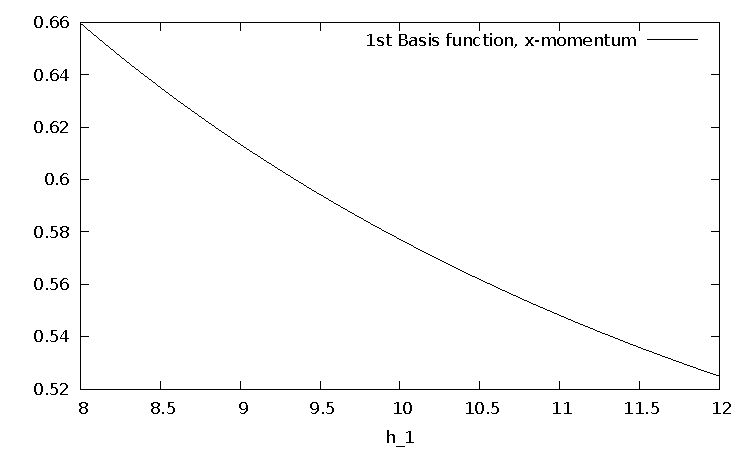
\includegraphics[scale=\zoomfactor]{{{magnitude_10_heights_momentums/y_12.0_9.0_2.0_-3.0_1.0_3.0_2.0_-3.0f00}}}
  }
  \quad \subfloat[] {
    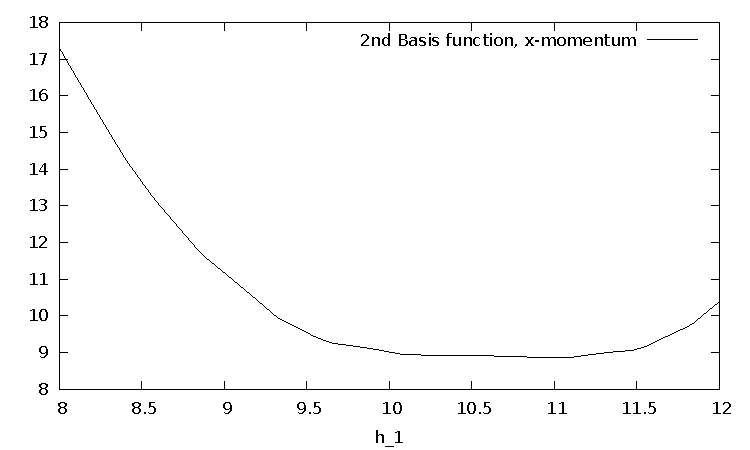
\includegraphics[scale=\zoomfactor]{{{magnitude_10_heights_momentums/y_12.0_9.0_2.0_-3.0_1.0_3.0_2.0_-3.0f02}}}
  }

magnitude_1000_heightsmomentums/y_1002.0_999.0_2.0_-3.0_1.0_3.0_2.0_-3.0f00.pdf

  \quad \subfloat[] {
    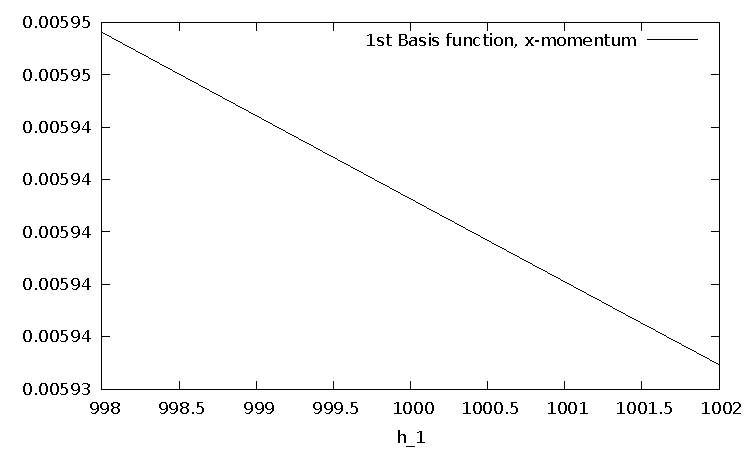
\includegraphics[scale=\zoomfactor]{{{magnitude_1000_heightsmomentums/y_1002.0_999.0_2.0_-3.0_1.0_3.0_2.0_-3.0f00}}}
  }
  \quad \subfloat[] {
    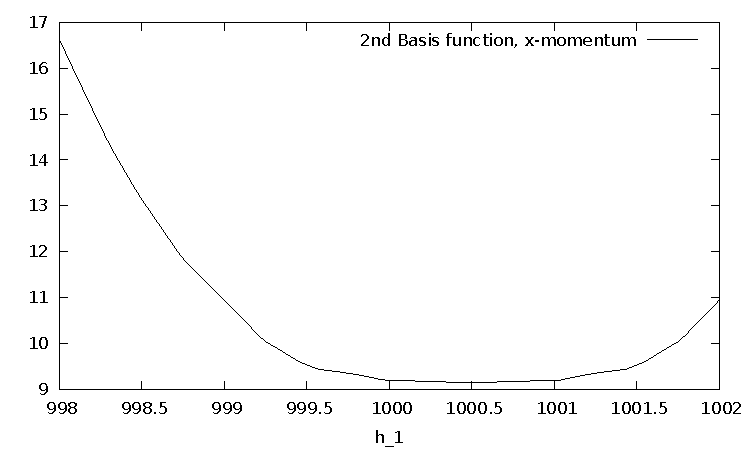
\includegraphics[scale=\zoomfactor]{{{magnitude_1000_heightsmomentums/y_1002.0_999.0_2.0_-3.0_1.0_3.0_2.0_-3.0f02}}}
  }
\caption{}
\label{fig:magnitude_10_heights_momentums}
\end{figure}

%%% Local Variables:
%%% TeX-master: "../results.tex"
%%% End:
